\documentclass[%
  english,
  hyperref={pdfpagelabels=false},
  aspectratio=1610]{beamer}

\usepackage{lmodern}  % nicer fonts
\usepackage[utf8]{inputenc}
\usepackage[T1]{fontenc}

\mode<handout>{
  \usepackage{pgf}
  \usepackage{pgfpages}
  \pgfpagesuselayout{2 on 1}[a4paper,border shrink=5mm]
}
\mode<presentation>{
  \usetheme{Juelich}
}

\usepackage[english]{babel}
\usepackage[scaled]{helvet}
\usepackage{graphics}

\usepackage{listings}  % for source code display

\usepackage{hyperref}

\title{PyPinT}
\subtitle{Towards a framework for rapid prototyping of iterative parallel-in-time algorithms}
\author{Dieter Moser, Torbjörn Klatt, Dr. Robert Speck
  <\href{mailto:d.moser@fz-juelich.de}{\{d.moser,t.klatt,r.speck\}@fz-juelich.de}>%
}
\institute{3rd Workshop on Parallel-in-Time Integration Methods}
\date{May 28, 2014}
\setbeamertemplate{slide counter}[showall]


\begin{document}
\maketitle

\begin{frame}
  \frametitle{Overview}
  \begin{enumerate}
    \item Recap of existing Parallel-in-Time Algorithms
    \item The \emph{PyPinT} Framework Explained
    \item Goals
    \item Proof of Concept --- Examples Analyzed
  \end{enumerate}
\end{frame}


%%%%%%%%%%%%%%%%%%%%%%%%%%%%%%%%%%%%%%%%%%%%%%%%%%%%%%%%%%%%%%%%%%%%%%%%%%%%%%%%
\part{Existing Parallel-in-Time Approaches}
\makepart


\begin{frame}
  \frametitle{Parareal}
  \framesubtitle{\scriptsize\normalfont Reference}
  \begin{columns}[T]
    \begin{column}{4cm}
      \begin{itemize}
	\item coarse $\mathcal{\textcolor{blue}{G}}$ and fine $\mathcal{\textcolor{red}{F}}$ propagators make parareal
	  flexible and \textcolor{orange}{modular}
	\item an initial value is improved \textcolor{orange}{iteratively}
	\item order is controllable through the fine propagator $\mathcal{\textcolor{red}{F}}$ 
      \end{itemize}
    \end{column}
    \begin{column}{8cm}
      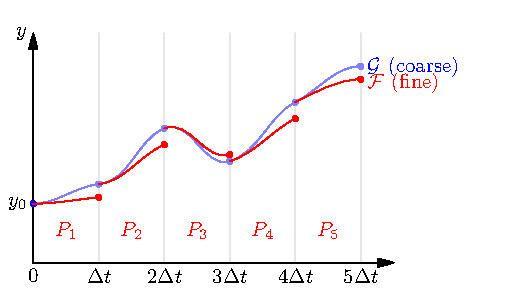
\includegraphics[width=8cm]{src/parareal_overview}

      \vspace*{-0.2cm} \hfill {\tiny [Courtesy of M.~Emmett, LBNL]}\\[0.1cm]

  \end{column}
\end{columns}
              \begin{align*}
                  \textcolor{orange}{y_{m+1}^{k+1}} = \textcolor{red}{\mathcal{F}(y_m^k)} + \textcolor{blue}{\mathcal{G}(y_m^{k+1})} - \textcolor{blue}{\mathcal{G}(y_m^k)}
              \end{align*}

\end{frame}

\begin{frame}
  \frametitle{IDC and DC}

  \begin{columns}[T]
    \begin{column}{6cm}
    \begin{align*}
      y'(t) = f\left( y\left( t \right),t \right),\quad y\left( 0 \right)= y_{0}
    \end{align*}
    Using the residual
    \begin{align*}
	r(t) &= f\left( t, \tilde y\left( t \right) \right) - \tilde y\left( t \right)
      \end{align*}
    to compute the error
    \begin{align*}
	e'(t) &= f(t,\tilde u + e) - f\left( t, \tilde y \right) + r'\left( t \right)\\
	e(0)  &= 0
    \end{align*}
    for the next update
    \begin{align*}
      \tilde y_{j+1} = \tilde y_{j} + e_{j}
    \end{align*}
    

    \end{column}
    \begin{column}{6cm}
    
     \begin{align*}
      y'(t) = f\left( y\left( t \right),t \right),\quad y\left( 0 \right)= y_{0}
    \end{align*}
    Using the residual
    \begin{align*}
	r(t) &= f\left( t, \tilde y\left( t \right) \right) - \tilde y\left( t \right)
      \end{align*}
    to compute the error
    \begin{align*}
	e'(t) &= f(t,\tilde u + e) - f\left( t, \tilde y \right) + r'\left( t \right)\\
	e(0)  &= 0
    \end{align*}
    for the next update
    \begin{align*}
      \tilde y_{j+1} = \tilde y_{j} + e_{j}
    \end{align*}
    



  \end{column}
\end{columns}


\end{frame}

\begin{frame}
  \frametitle{RIDC}
\end{frame}


\begin{frame}
  \frametitle{RIDC}
\end{frame}


\begin{frame}
  \frametitle{PFASST}
  \framesubtitle{Building Blocks}
  
  \begin{picture}(1,1)
    \put(50,-125){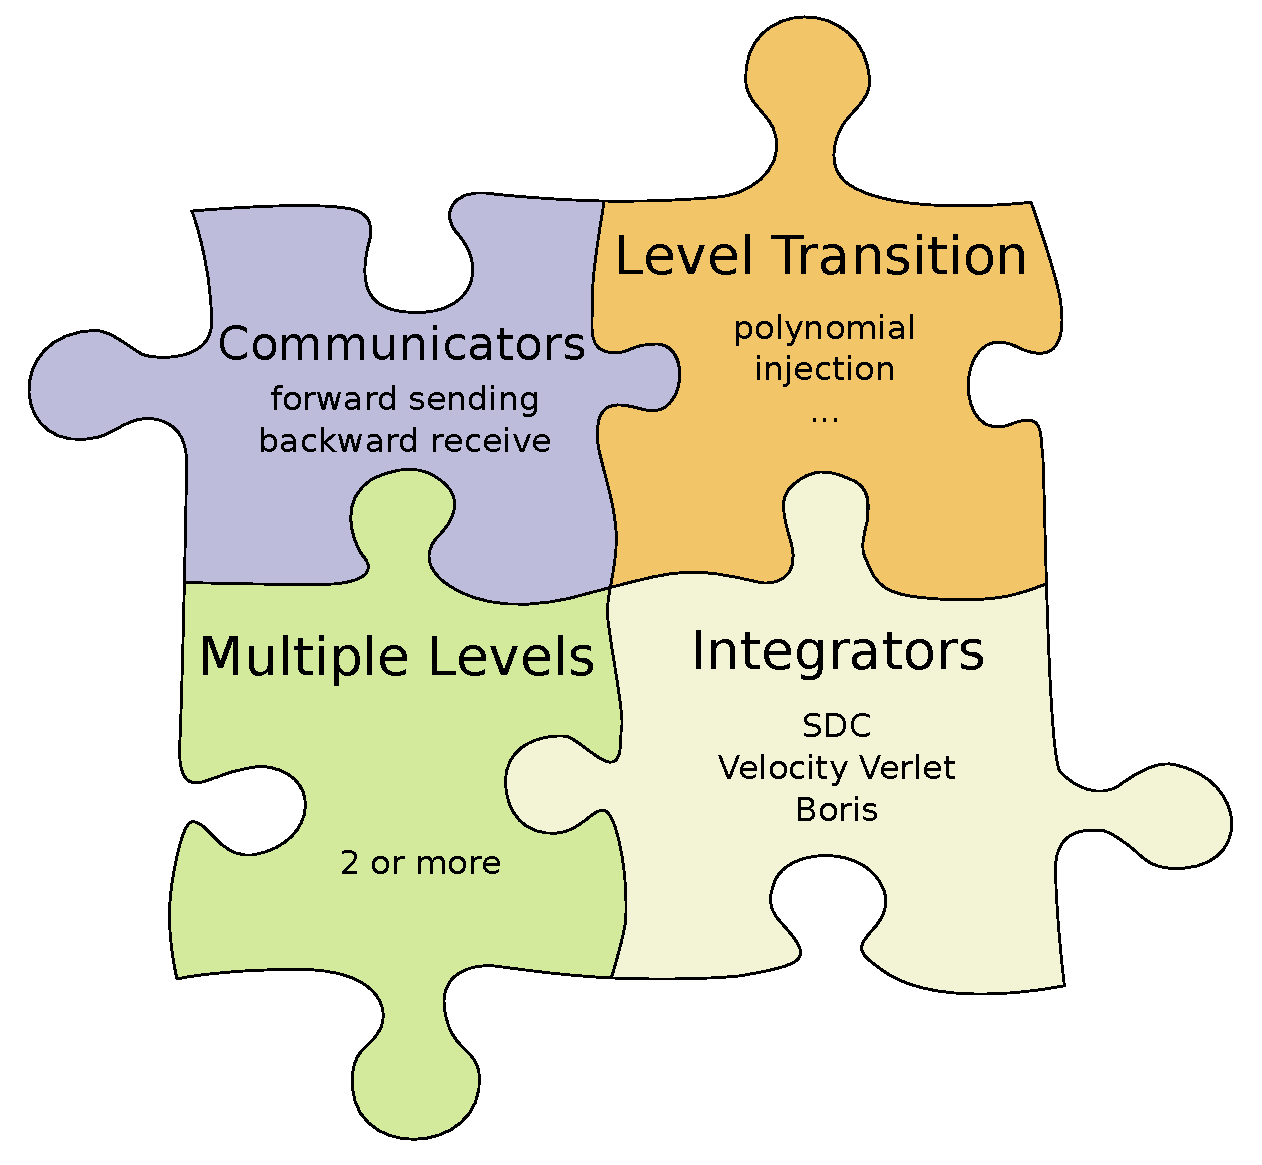
\includegraphics[height=9.5cm]{src/pfasst_blocks.pdf}}
  \end{picture}

\end{frame}


%%%%%%%%%%%%%%%%%%%%%%%%%%%%%%%%%%%%%%%%%%%%%%%%%%%%%%%%%%%%%%%%%%%%%%%%%%%%%%%%
\part{The PyPinT Framework Explained}
\makepart

\begin{frame}
  \frametitle{Basic Concept}
  \begin{itemize}
    \item \emph{Python} {\color{fzjgray50}\scriptsize $\geq$3.2} as language of choice\\
      {\scriptsize for ease of use and extensibility (cf. \emph{NumPy}, \emph{SciPy})}
    \item well-conceived and intuitive abstract interfaces\\
      {\scriptsize for reusable code ensuring DRY principle}
    \item modular building blocks\\
      {\scriptsize for fast exchange of algorithms' building blocks}
    \item integrated analyzation tools\\
      {\scriptsize for introspection and plotting (cf. \emph{matplotlib})}
    \item usage of a sophisticated testing framework\\
      {\scriptsize nobody writes bug-free code}
  \end{itemize}
  
  \begin{picture}(1,1)
    \put(260,150){
\includegraphics[height=1.25cm]{src/python_logo.png}}
    \put(290,135){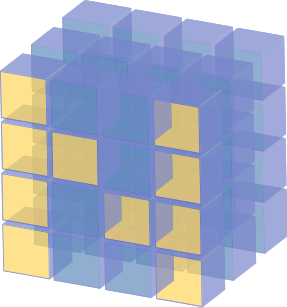
\includegraphics[height=0.75cm]{src/numpy_logo.png}}
    \put(325,135){
\includegraphics[height=0.75cm]{src/scipy_logo.png}}
    \put(290,80){
\includegraphics[height=1.1cm]{src/puzzle.png}}
    \put(255,50){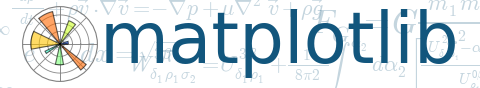
\includegraphics[height=0.75cm]{src/matplotlib_logo.png}}
  \end{picture}
\end{frame}

\begin{frame}
  \frametitle{Modules}
  \framesubtitle{Abstract Modelling of PinT Algorithms}
  \vspace{-5em}
  \begin{columns}[T]
    \begin{column}{5cm}
      \color{fzjblue50}%
      \texttt{pypint}\\
      \color{fzjgray30}%
      \hspace{0.75em}\texttt{\textasciitilde.problems}\\
      \hspace{0.75em}\texttt{\textasciitilde.solvers}\\
      \hspace{0.75em}\texttt{\textasciitilde.integrators}\\
      \hspace{0.75em}\texttt{\textasciitilde.communicators}\\
      \hspace{0.75em}\texttt{\textasciitilde.multi\_level\_providers}\\
      \hspace{0.75em}\texttt{\textasciitilde.solutions}\\
      \hspace{0.75em}\texttt{\textasciitilde.plugins}
    \end{column}
    \begin{column}{10cm}      
      \begin{picture}(1,1)
        \put(50,-110){
\includegraphics[width=5cm]{src/puzzle.png}}
      \end{picture}
    \end{column}
  \end{columns}
\end{frame}

\begin{frame}
  \frametitle{Modules}
  \framesubtitle{Abstract Modelling of PinT Algorithms}
  \vspace{-5em}
  \begin{columns}[T]
    \begin{column}{5cm}
      \color{fzjblue50}%
      \texttt{pypint}\\
      \color{fzjblue50}%
      \hspace{0.75em}\texttt{\textasciitilde.problems}\\
      \color{fzjgray30}%
      \hspace{0.75em}\texttt{\textasciitilde.solvers}\\
      \hspace{0.75em}\texttt{\textasciitilde.integrators}\\
      \hspace{0.75em}\texttt{\textasciitilde.communicators}\\
      \hspace{0.75em}\texttt{\textasciitilde.multi\_level\_providers}\\
      \hspace{0.75em}\texttt{\textasciitilde.solutions}\\
      \hspace{0.75em}\texttt{\textasciitilde.plugins}
    \end{column}
    \begin{column}{10cm}
      \begin{itemize}
        \item interfaces for problem setups
        \item generic problem with specializations via mixins
      \end{itemize}
      
      \begin{picture}(1,1)
        \put(25,-120){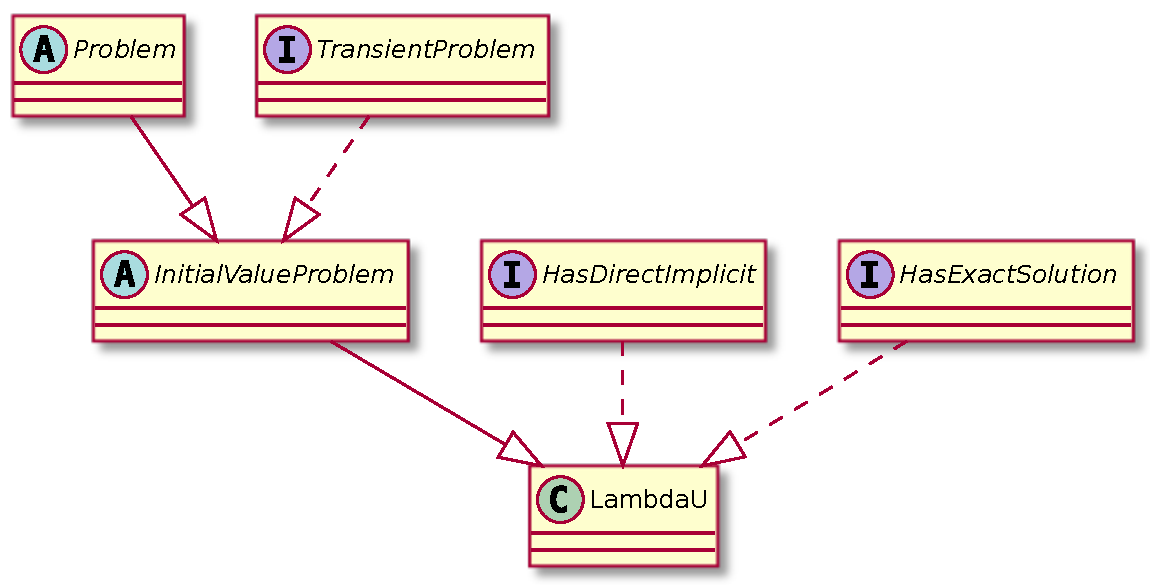
\includegraphics[width=8.5cm]{src/problem_interfaces.pdf}}
      \end{picture}
    \end{column}
  \end{columns}
\end{frame}

\begin{frame}
  \frametitle{Modules}
  \framesubtitle{Abstract Modelling of PinT Algorithms}
  \vspace{-5em}
  \begin{columns}[T]
    \begin{column}{5cm}
      \color{fzjblue50}%
      \texttt{pypint}\\
      \color{fzjgray30}%
      \hspace{0.75em}\texttt{\textasciitilde.problems}\\
      \color{fzjblue50}%
      \hspace{0.75em}\texttt{\textasciitilde.solvers}\\
      \color{fzjgray30}%
      \hspace{0.75em}\texttt{\textasciitilde.integrators}\\
      \hspace{0.75em}\texttt{\textasciitilde.communicators}\\
      \hspace{0.75em}\texttt{\textasciitilde.multi\_level\_providers}\\
      \hspace{0.75em}\texttt{\textasciitilde.solutions}\\
      \hspace{0.75em}\texttt{\textasciitilde.plugins}
    \end{column}
    \begin{column}{10cm}
      \begin{itemize}
        \item interfaces for iterative time solvers
        \item providing generic building blocks of solvers
      \end{itemize}
      
      \begin{picture}(1,1)
        \put(50,-125){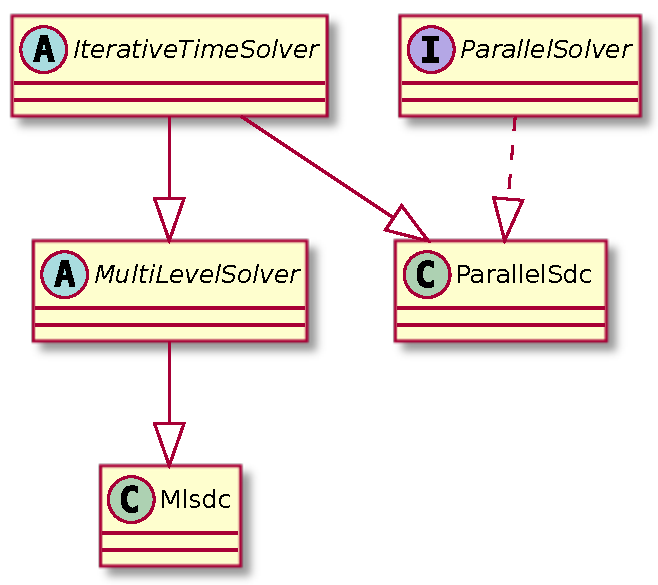
\includegraphics[height=4.5cm]{src/solvers_interfaces.pdf}}
      \end{picture}
    \end{column}
  \end{columns}
\end{frame}

\begin{frame}
  \frametitle{Modules}
  \framesubtitle{Abstract Modelling of PinT Algorithms}
  \vspace{-5em}
  \begin{columns}[T]
    \begin{column}{5cm}
      \color{fzjblue50}%
      \texttt{pypint}\\
      \color{fzjgray30}%
      \hspace{0.75em}\texttt{\textasciitilde.problems}\\
      \hspace{0.75em}\texttt{\textasciitilde.solvers}\\
      \color{fzjblue50}%
      \hspace{0.75em}\texttt{\textasciitilde.integrators}\\
      \color{fzjgray30}%
      \hspace{0.75em}\texttt{\textasciitilde.communicators}\\
      \hspace{0.75em}\texttt{\textasciitilde.multi\_level\_providers}\\
      \hspace{0.75em}\texttt{\textasciitilde.solutions}\\
      \hspace{0.75em}\texttt{\textasciitilde.plugins}
    \end{column}
    \begin{column}{10cm}
      \begin{itemize}
        \item providers of various quadrature nodes and weight functions\\
          {\scriptsize e.g. Gauss-Lobatto, Gauss-Legendre, polynomial, etc.\\}
        \item providers aggregated in integrators\\
          {\scriptsize for intuitive \texttt{.integrate(data, from\_node=0, to\_node='last')} method\\}
      \end{itemize}
      
      \begin{picture}(1,1)
        \put(25,-100){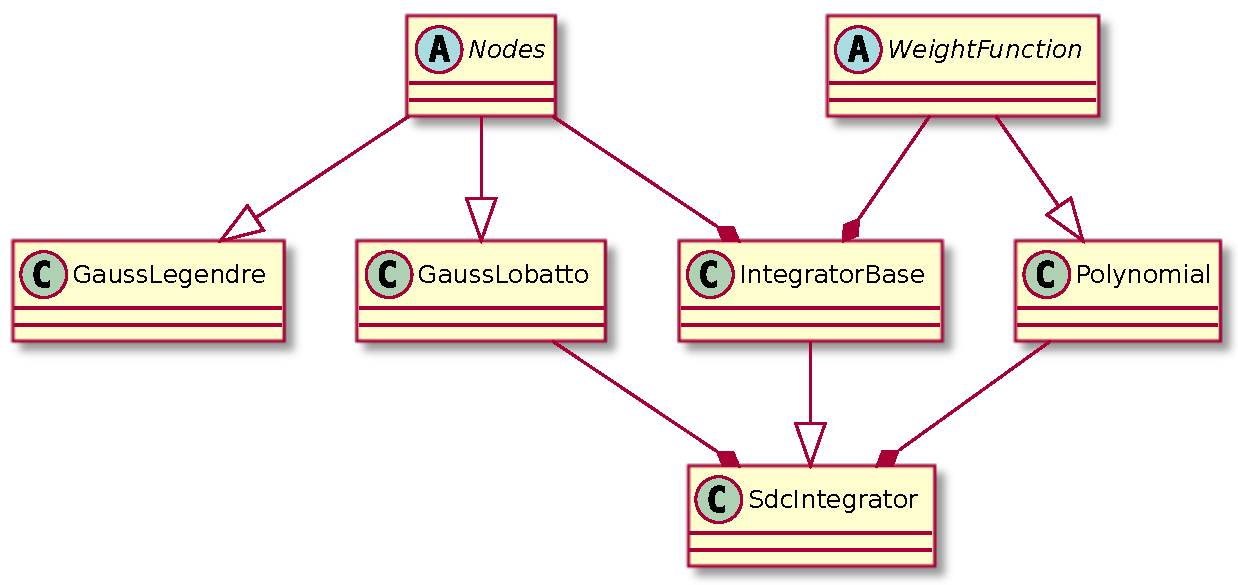
\includegraphics[height=3.75cm]{src/integrators_interfaces.pdf}}
      \end{picture}
    \end{column}
  \end{columns}
\end{frame}

\begin{frame}
  \frametitle{Modules}
  \framesubtitle{Abstract Modelling of PinT Algorithms}
  \vspace{-5em}
  \begin{columns}[T]
    \begin{column}{5cm}
      \color{fzjblue50}%
      \texttt{pypint}\\
      \color{fzjgray30}%
      \hspace{0.75em}\texttt{\textasciitilde.problems}\\
      \hspace{0.75em}\texttt{\textasciitilde.solvers}\\
      \hspace{0.75em}\texttt{\textasciitilde.integrators}\\
      \color{fzjblue50}%
      \hspace{0.75em}\texttt{\textasciitilde.communicators}\\
      \color{fzjgray30}%
      \hspace{0.75em}\texttt{\textasciitilde.multi\_level\_providers}\\
      \hspace{0.75em}\texttt{\textasciitilde.solutions}\\
      \hspace{0.75em}\texttt{\textasciitilde.plugins}
    \end{column}
    \begin{column}{10cm}
      \begin{itemize}
        \item generic abstract interfaces for communication patterns\\
          {\scriptsize e.g. implemented as \emph{forward sending}, etc.\\}
        \item extendable basic message buffer\\
          {\scriptsize holding data, solver flags and other meta information\\}
      \end{itemize}
      
      \begin{picture}(1,1)
        \put(50,-75){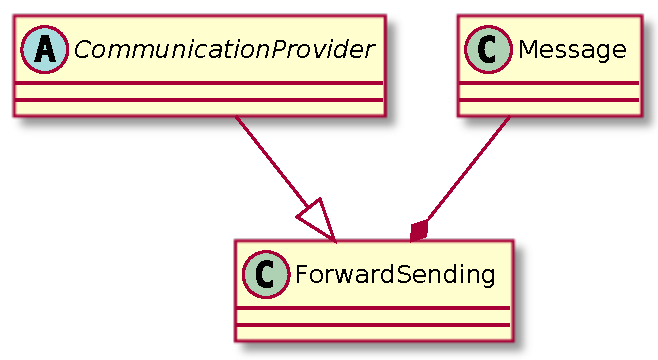
\includegraphics[height=2.5cm]{src/communicators_interfaces.pdf}}
      \end{picture}
    \end{column}
  \end{columns}
\end{frame}

\begin{frame}
  \frametitle{Modules}
  \framesubtitle{Abstract Modelling of PinT Algorithms}
  \vspace{-5em}
  \begin{columns}[T]
    \begin{column}{5cm}
      \color{fzjblue50}%
      \texttt{pypint}\\
      \color{fzjgray30}%
      \hspace{0.75em}\texttt{\textasciitilde.problems}\\
      \hspace{0.75em}\texttt{\textasciitilde.solvers}\\
      \hspace{0.75em}\texttt{\textasciitilde.integrators}\\
      \hspace{0.75em}\texttt{\textasciitilde.communicators}\\
      \color{fzjblue50}%
      \hspace{0.75em}\texttt{\textasciitilde.multi\_level\_providers}\\
      \color{fzjgray30}%
      \hspace{0.75em}\texttt{\textasciitilde.solutions}\\
      \hspace{0.75em}\texttt{\textasciitilde.plugins}
    \end{column}
    \begin{column}{10cm}
      \begin{itemize}
        \item abstract interface for generic level transitions\\
          {\scriptsize e.g. \emph{full weighting}, \emph{injection}, \emph{Legendre-polynomial integration} etc.\\}
        \item containers for multiple levels\\
          {\scriptsize providing access to integrators of each level\\}
        \item unified generic interface for transitions between levels\\
          {\scriptsize via methods \texttt{.restringate(data, fine\_id, coarse\_id)} and\\[-0.5em]
           \texttt{.prolongate(data, coarse\_id, fine\_id)}}
      \end{itemize}
      
      \begin{picture}(1,1)
        \put(25,-85){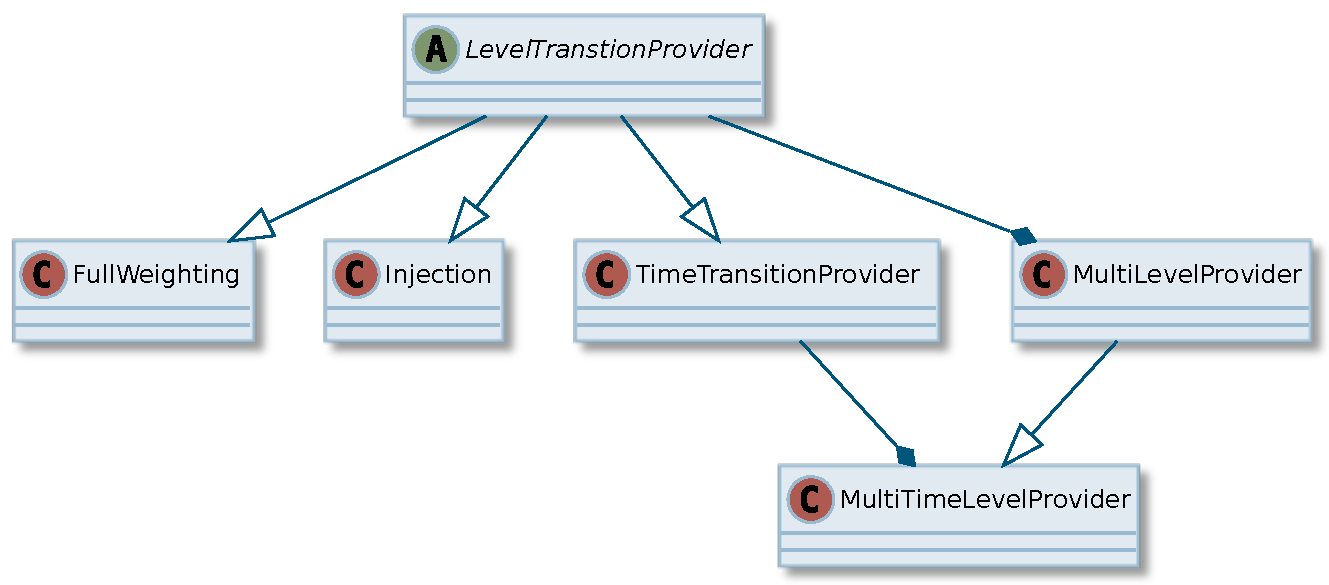
\includegraphics[height=3.5cm]{src/multi_level_providers_interfaces.pdf}}
      \end{picture}
    \end{column}
  \end{columns}
\end{frame}

\begin{frame}
  \frametitle{Modules}
  \framesubtitle{Abstract Modelling of PinT Algorithms}
  \vspace{-5em}
  \begin{columns}[T]
    \begin{column}{5cm}
      \color{fzjblue50}%
      \texttt{pypint}\\
      \color{fzjgray30}%
      \hspace{0.75em}\texttt{\textasciitilde.problems}\\
      \hspace{0.75em}\texttt{\textasciitilde.solvers}\\
      \hspace{0.75em}\texttt{\textasciitilde.integrators}\\
      \hspace{0.75em}\texttt{\textasciitilde.communicators}\\
      \hspace{0.75em}\texttt{\textasciitilde.multi\_level\_providers}\\
      \color{fzjblue50}%
      \hspace{0.75em}\texttt{\textasciitilde.solutions}\\
      \color{fzjgray30}%
      \hspace{0.75em}\texttt{\textasciitilde.plugins}
    \end{column}
    \begin{column}{10cm}
      \begin{itemize}
        \item containers for solution data + meta information\\
          {\scriptsize e.g. time-node/step-wise, trajectory (consecutive time nodes)\\}
        \item container interface for complete solutions\\
          {\scriptsize e.g. only last time node of last iteration or all nodes of all iterations\\}
      \end{itemize}
      
      \begin{picture}(1,1)
        \put(60,-115){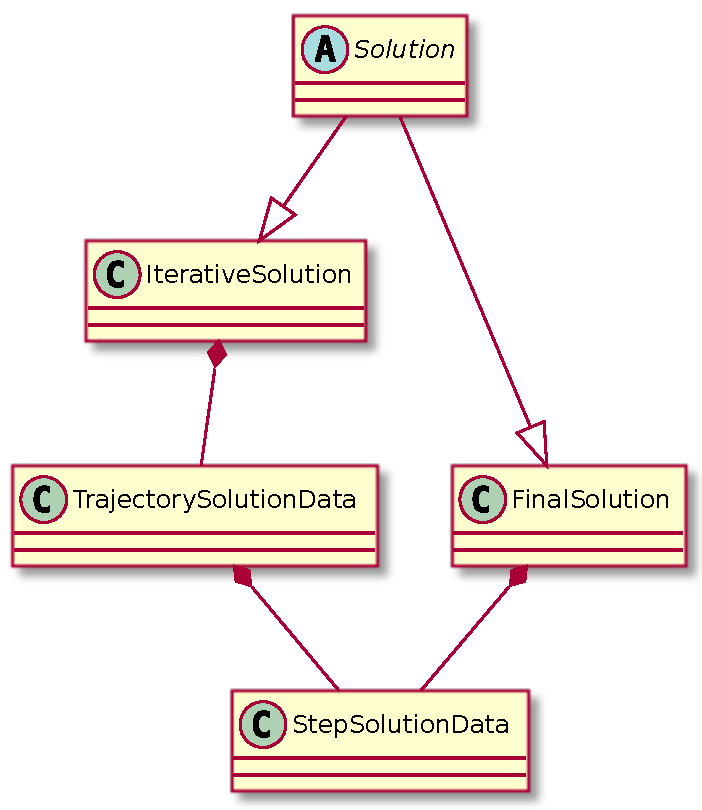
\includegraphics[height=4.5cm]{src/solutions_interfaces.pdf}}
      \end{picture}
    \end{column}
  \end{columns}
\end{frame}

\begin{frame}
  \frametitle{Modules}
  \framesubtitle{Abstract Modelling of PinT Algorithms}
  \vspace{-5em}
  \begin{columns}[T]
    \begin{column}{5cm}
      \color{fzjblue50}%
      \texttt{pypint}\\
      \color{fzjgray30}%
      \hspace{0.75em}\texttt{\textasciitilde.problems}\\
      \hspace{0.75em}\texttt{\textasciitilde.solvers}\\
      \hspace{0.75em}\texttt{\textasciitilde.integrators}\\
      \hspace{0.75em}\texttt{\textasciitilde.communicators}\\
      \hspace{0.75em}\texttt{\textasciitilde.multi\_level\_providers}\\
      \hspace{0.75em}\texttt{\textasciitilde.solutions}\\
      \color{fzjblue50}%
      \hspace{0.75em}\texttt{\textasciitilde.plugins}
    \end{column}
    \begin{column}{10cm}
      \begin{itemize}
        \item containers for solution data + meta information\\
          {\scriptsize e.g. time-node/step-wise, trajectory (consecutive time nodes)\\}
        \item container interface for complete solutions\\
          {\scriptsize e.g. only last time node of last iteration or all nodes of all iterations\\}
      \end{itemize}
      
      \begin{picture}(1,1)
        \put(10,-100){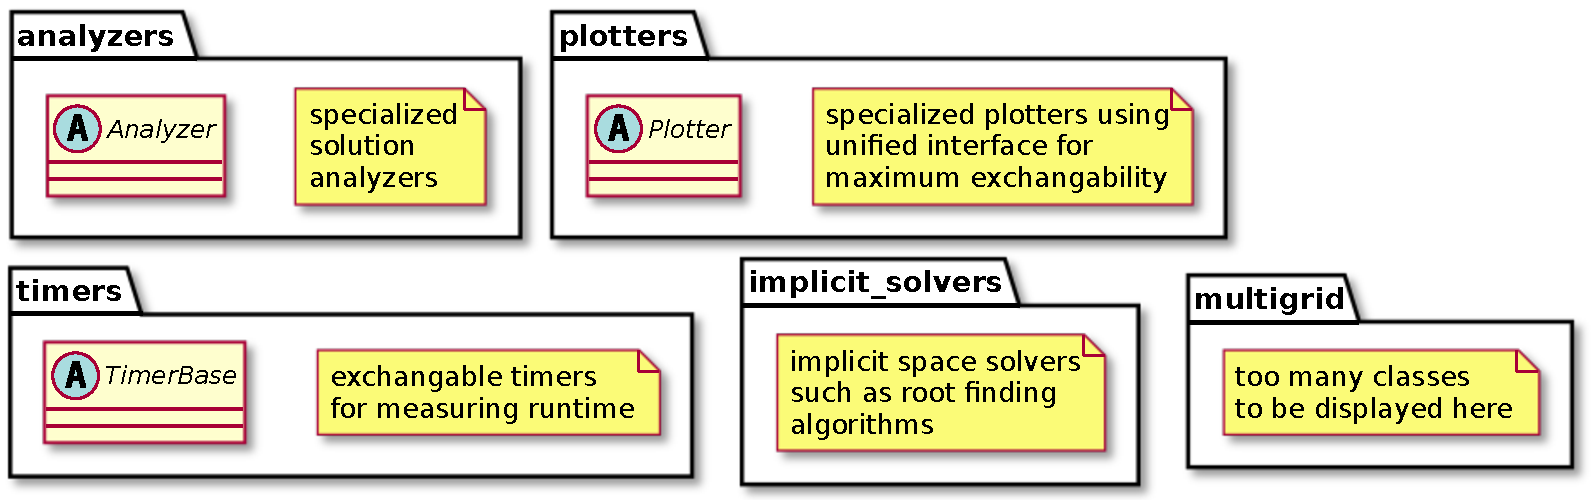
\includegraphics[width=9cm]{src/plugins_tree.pdf}}
      \end{picture}
    \end{column}
  \end{columns}
\end{frame}


%%%%%%%%%%%%%%%%%%%%%%%%%%%%%%%%%%%%%%%%%%%%%%%%%%%%%%%%%%%%%%%%%%%%%%%%%%%%%%%%
\part{Goals for PyPinT}
\makepart

\begin{frame}
  \frametitle{Goals for PyPinT}
  
  \begin{itemize}
    \item<1-> providing generic framework for PINT algorithms\\
      {\onslide<2->\color{fzjblue50}$\Rightarrow$ easy comparability of different algorithms' building blocks\\[1.5em]}
    \item<3-> intuitive user-expandability through well-defined interfaces\\
      {\onslide<4->\color{fzjblue50}$\Rightarrow$ fast exchangability and prototyping of different building blocks\\[1.5em]}
    \item<5-> well-tested and well-documented implementations of PINT algorithms\\
      {\onslide<6->\color{fzjblue50}$\Rightarrow$ suited for educational use\\[1.5em]}
    \item<7-> open-source hosted on 
\includegraphics[height=1em]{src/GitHub-Mark-32px.png}~GitHub\\
      {\onslide<8->\color{fzjblue50}$\Rightarrow$ reaching young \& rising developers and scientists promoting PINT algorithms\\[1.5em]}
  \end{itemize}
\end{frame}


%%%%%%%%%%%%%%%%%%%%%%%%%%%%%%%%%%%%%%%%%%%%%%%%%%%%%%%%%%%%%%%%%%%%%%%%%%%%%%%%
\part{Proof of Concept}
\makepart

\begin{frame}
  \frametitle{Implementation of SDC and MLSDC}
  \framesubtitle{Stability Regions of $u'(x,t)=\lambda u(x,t)$, $t\in[0,1]$}
  \begin{columns}[T]
    \begin{column}{7cm}
      \vspace{-7.75em}
      \centering
      {\color{fzjblue50}SDC}
      \begin{picture}(1,1)
%         \put(-50,-88){\includegraphics[height=3cm]{src/sdc_p3.png}}
        \put(-35,-95){\tiny $3$ Gauss-Lobatto nodes}
%         \put(-50,-188){\includegraphics[height=3cm]{src/sdc_p5.png}}
        \put(-35,-195){\tiny $5$ Gauss-Lobatto nodes}
      \end{picture}
    \end{column}
    \begin{column}{7cm}
      \vspace{-7.75em}
      \centering
      {\color{fzjblue50}MLSDC}
      \begin{picture}(1,1)
%         \put(-65,-88){\includegraphics[height=3cm]{src/mlsdc_p3.png}}
        \put(-50,-95){\tiny $3$ Gauss-Lobatto nodes}
%         \put(-65,-188){\includegraphics[height=3cm]{src/mlsdc_p5.png}}
        \put(-50,-195){\tiny $5$ Gauss-Lobatto nodes}
      \end{picture}
    \end{column}
  \end{columns}
\end{frame}


%%%%%%%%%%%%%%%%%%%%%%%%%%%%%%%%%%%%%%%%%%%%%%%%%%%%%%%%%%%%%%%%%%%%%%%%%%%%%%%%
\begin{frame}
  \frametitle{~}
  \begin{center}
    {\huge Thank you for your attention!}\par
    \bigskip
    \bigskip
    \bigskip
    {\Large Questions?}\par
    {\scriptsize\color{fzjgray50}(now or later)}\par
    \bigskip
    {\scriptsize \emph{PyPinT} is on 
\includegraphics[height=1em]{src/GitHub-Mark-32px.png}~GitHub: \url{https://github.com/Parallel-in-Time/PyPinT}}
    \bigskip
    \begin{columns}
      \tiny
      \begin{column}{0.09\textwidth}
      \end{column}
      \begin{column}{0.3\textwidth}
        Dieter Moser\\
        Juelich Supercomputing Centre\\
        Building 16.3, Room 022\\
        Tel: +49~2461~61~96453\\
        eMail: \href{mailto:d.moser@fz-juelich.de}{d.moser@fz-juelich.de}
      \end{column}
      \begin{column}{0.3\textwidth}
        Torbjörn Klatt\\
        Juelich Supercomputing Centre\\
        Building 16.3, Room 022\\
        Tel: +49~2461~61~96452\\
        eMail: \href{mailto:t.klatt@fz-juelich.de}{t.klatt@fz-juelich.de}
      \end{column}
      \begin{column}{0.3\textwidth}
        Dr. Robert Speck~*\\
        Juelich Supercomputing Centre\\
        Building 16.3, Room 131\\
        Tel: +49~2461~61~1644\\
        eMail: \href{mailto:r.speck@fz-juelich.de}{r.speck@fz-juelich.de}
      \end{column}
      \begin{column}{0.01\textwidth}
      \end{column}
    \end{columns}
  \end{center}
  \vfill
  {\tiny * corresponding author}
\end{frame}

\end{document}
